\selectlanguage{german}
\subsection{Muss - Anforderungen}

\subsubsection{Docker}
\nameref{subsec:docker} ist ein Tool, das Anwendungen in kompakten, tragbaren \nameref{subsec:container} organisiert und ausführt. Diese \nameref{subsec:container} sind von der Umgebung isoliert, in der sie laufen, was bedeutet, dass sie konsistent funktionieren, unabhängig davon, wo sie eingesetzt werden. Für dieses Self-Hosted Projekt auf einem \nameref{subsec:pi} bietet \nameref{subsec:docker} die Möglichkeit, verschiedene Dienste und Anwendungen ohne Konflikte nebeneinander auszuführen.

Durch die Nutzung von \nameref{subsec:docker} kann man sicherstellen, dass jede Anwendung und jeder Service seine eigene Umgebung hat, was die Sicherheit verbessert und es einfacher macht, Updates und Änderungen durchzuführen, ohne andere Teile des Systems zu beeinträchtigen. \nameref{subsec:docker} ist besonders wertvoll, wenn man mehrere unterschiedliche Anwendungen auf einem einzigen \nameref{subsec:pi} hosten möchte, da es die Verwaltung deutlich vereinfacht\cite{Docker}.

\subsubsection{Ubuntu 22.04 (LTS)}
\nameref{subsec:ubuntu}, ist einer der beliebten Linux-Betriebssystemen. Sie bietet langfristige Unterstützung bis April 2027, was sie zu einer zuverlässigen Wahl für das Patient Monitoring System Projekt macht. Diese Version ist benutzerfreundlich und ideal für eine Vielzahl von Anwendungen, von Lernen und Experimentieren bis hin zu ernsthaften technischen Projekten \cite{Ubuntu}.

\subsubsection{Dynamisches DNS-Management (ddclient)}
Der \nameref{subsec:ddclient} ist ein Tool, das speziell für die Aktualisierung dynamischer DNS-Einträge entwickelt wurde. Es ermöglicht es Geräten wie dem \nameref{subsec:pi}, die oft keine feste IP-Adresse haben, dennoch unter einem konstanten Domainnamen erreichbar zu sein. Durch die automatische Überwachung und Aktualisierung der sich ändernden öffentlichen IP-Adresse des \nameref{subsec:pi} sorgt \nameref{subsec:ddclient} dafür, dass der Pi auch nach einem IP-Wechsel durch den Internetdienstanbieter zugänglich bleibt. Diese Funktion ist besonders wertvoll für die Verwendung des \nameref{subsec:pi} als Home-Server für Anwendungen wie Webhosting, Dateifreigaben oder Überwachungsdienste. Die Installation und Konfiguration von \nameref{subsec:ddclient} ist unkompliziert und erfolgt über die Kommandozeile \cite{Ddclient}.

\subsubsection{Fail2ban}
\nameref{subsec:f2b} ist ein entscheidendes Werkzeug zur Absicherung, die dazu dient, einen Server vor unautorisierten Zugriffsversuchen und \nameref{subsec:bruteforce} zu schützen. Durch die Überwachung von Logdateien erkennt \nameref{subsec:f2b} auffällige Anmeldeversuche und blockiert die zugehörigen IP-Adressen automatisch für eine vordefinierte Zeitdauer. Mit \nameref{subsec:f2b} kann beispielsweise die IP-Adresse eines Geräts, das wiederholt versucht, ohne die korrekten Anmeldedaten eine Verbindung zum Server herzustellen, blockiert werden. Es lässt sich so konfigurieren, dass jede IP-Adresse, die mehr als dreimal pro Tag versucht, sich zu verbinden, gesperrt wird \cite{Fail2ban}. Diese Funktion ist besonders wichtig für die Minimierung von potenziellen Sicherheitsrisiken. Im Rahmen unseres Projekts auf dem \nameref{subsec:pi} wird \nameref{subsec:f2b} eine kritische Rolle spielen, indem es dazu beiträgt, die Zugriffskontrolle auf unsere Dienste wie \nameref{subsec:ssh} verstärken.

\subsubsection{MQTT / MQTT-Client}
Das System besteht aus mehreren verschiedenen Komponenten, die miteinander kommunizieren. Diese Kommunikation erfolgt über einen Message-Broker und das Protokoll ''\nameref{subsec:mqtt}'' \cite{MQTT}. Um das Protokoll nutzen zu können, benötigt es einen MQTT-Message Broker und Clients, die ihre Nachrichten an diesen schicken, damit sie an die Clients verteilt werden, die darum gebeten haben, Nachrichten eines Topics zu erhalten.

\subsubsection{SMTP-Server / SMTP-Client}
Zu Zwecken der Protokollierung und Dokumentation sendet das System zusätzlich zu einem \nameref{subsec:alarm} eine Mail an einen eigenen Mail-Server. Dieser Mail-Server empfängt über das \nameref{subsec:smtp}-Protokoll Mails. Dafür wird ein \nameref{subsec:mailcow}-Server eingerichtet \cite{Mailcow}. Hierfür müssen auch \nameref{subsec:dnsentries} angepasst werden.

\subsubsection{Raspberry und Raspberry Pi} \label{sec:raspi}
Für das Projekt wird der \nameref{subsec:pi} gewählt, da dieser eine einfache Anbindung mit einer Kamera erlaubt \cite{Raspberry} \cite{Raspberry_camera}. Der \nameref{subsec:pi} ermöglicht es, Microcontroller und Kamera in einem kompakten Gehäuse unterzubringen. Es gibt zwei Raspberry Pis, die eine Detektion durchführen (siehe Abb. \ref{fig:patient_monitoring}). Ein Raspberry Pi mit Raspberry Pi Kamera übernimmt die \nameref{subsec:beddetection} und ein weiterer Raspberry Pi mit Kamera übernimmt die \nameref{subsec:falldetection} Ein dritter Raspberry Pi wird verwendet, um einen \nameref{subsec:alarm} zu schalten.


\begin{figure}[H]
	\centering
	\begin{tikzpicture}[scale=0.8]
		
	
		\draw [-, dashed, gray] (4.5,1)-- (-4,1)--(-4,3.5) --(4.5,3.5) --(4.5,1);
		
			\node at (-2.8 ,3.2) {\scriptsize BED VIEW};
					
		\node[inner sep=0pt] (whitehead) at (2,2.5)
		{
\includegraphics[width=.05\textwidth]{images/camera.png}};
		
		\node[above] at (2.2,2.6) {\scriptsize Raspberry Pi und Kamera};
		
		\node[inner sep=0pt] (whitehead) at (0,2)
		{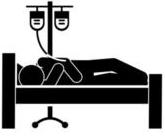
\includegraphics[width=.1\textwidth]{images/person_in_bed.png}};

			\node at (-2.6 ,-1) { \scriptsize ROOM VIEW};
	
			\draw [-, dashed, gray] (4.5,-0.6)-- (-4,-0.6)--(-4,-4) --(4.5, -4 ) --(4.5,-0.5);
		
		\node[inner sep=0pt] (whitehead) at (2,-1.5)
		{
\includegraphics[width=.05\textwidth]{images/camera.png}};
		

		
		\node[inner sep=0pt] (whitehead) at (-0.25,-1.25)
		{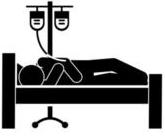
\includegraphics[width=.1\textwidth]{images/person_in_bed.png}};
		
		
		\node[inner sep=0pt] (whitehead) at (0,-2.25)
		{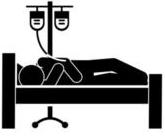
\includegraphics[width=.1\textwidth]{images/person_in_bed.png}};
		
	\node[inner sep=0pt] (whitehead) at (-0.5,-3.25)
		{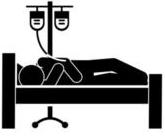
\includegraphics[width=.1\textwidth]{images/person_in_bed.png}};
		

	  \node[inner sep=0pt] (whitehead) at (4.0,0.25)
		{
\includegraphics[width=.08\textwidth]{images/server.png}};
		
				\node[below] at (2.2,-1.6) {\scriptsize Raspberry Pi und Kamera};
		
		\node[below] at (4.0,-0.1) {\scriptsize  Broker};
		
			
		
		\draw [-] (2,2.5)-- ( 3,2.5) -- (3,0.25) ;
		\draw [-] (2,-1.5)-- ( 3,-1.5) -- (3,0.25) ;
		\draw [-]  (3,0.25)  -- (3.8,0.25);

	    \draw [->]  (4.2 ,0.25) -- (5.0,0.25) -- (5.0,-1.5) -- (5.5,-1.5);
	     \draw [->]  (4.2 ,0.25) -- (5.0,0.25) -- (5.0,2.5) -- (5.5,2.5);
	
		\node at  (7.0,2.5) {\scriptsize Bed Detection};
		
		
		\node at  (7.0,-1.5) {\scriptsize Fall Detection};
		
		
	
	 	\draw [->]  (8.5 ,-1.5) -- (9.0,-1.5) -- (9,0.25) -- (9.5,0.25)  ;
	
		\draw [->]  (8.5, 2.5) -- (9.0,2.5) -- (9,0.25) -- (9.5,0.25) ;
		
		\node[inner sep=0pt] (whitehead) at (10.2,0.25)
		{
\includegraphics[width=.05\textwidth]{images/raspi.png}};
		
		\node[below] at (10.2,0.0) {\scriptsize Raspberry Pi };
		
		
		
	\end{tikzpicture}
	\caption{Darstellung des Systemaufbaus}
	\label{fig:patient_monitoring}
\end{figure}


\subsubsection{Fall Detektion}
Wie bereits in Abschnitt \ref{sec:raspi} erwähnt, führt ein \nameref{subsec:pi} mithilfe der Raspberry Pi Kamera die \nameref{subsec:falldetection} durch. Der \nameref{subsec:pi} überprüft, ob ein Patient hingefallen ist, was mithilfe des \nameref{subsec:yolo}-Frameworks realisiert wird \cite{Yolo}. Ziel ist es, das Modell auf dem \nameref{subsec:pi} zu implementieren, um den Bedarf an zusätzlichen Servern zu vermeiden.

\subsubsection{Matrix}
Ein \nameref{subsec:matrix}-Server ist vorhanden \cite{Matrix}. Über diesen Server werden Pfleger auch auf dem Handy benachrichtigt, wenn eine Alarmsituation eintritt. Dieser Kommunikationsdienst ermöglicht eine nahtlose und sichere Echtzeitkommunikation über verschiedene Geräte. Die Verwendung des Matrix-Protokolls garantiert dabei die Ende-zu-Ende-Verschlüsselung aller über-tragenen Daten, was die Vertraulichkeit und Sicherheit der sensiblen Patienteninformationen stärkt.

